\documentclass[a4paper,12pt]{article}
\usepackage[utf8]{inputenc}
\usepackage{url}
\usepackage{hyperref}
\usepackage[english,brazil]{babel}
\usepackage{comment}
\usepackage{bookmark}
\usepackage{graphicx}


\title{Estratégias de Sintetização de Voz utilizando Deep Learning para Leitura Humanizada de Textos}
\author{
  Aluno: Thomaz Diniz Pinto de Morais\\
  \texttt{thomaz.morais@ccc.ufcg.edu.br}
  \and
  Orientador: Herman Martins Gomes\\
  \texttt{hmg@dsc.ufcg.edu.br}
}
\date{}


\begin{document}	
	\maketitle
	\selectlanguage{english}
	\begin{abstract}
		Text-to-speech (TTS) is an extremely important tool in the pursuit of accessibility. It benefits not only people with visual impairments but also those with difficulties in reading comprehension. Recent advancements in deep learning enable the synthesis of voice with quality very close to recordings made by humans. In this study, we aim to replicate state-of-the-art techniques used to synthesize voices within the context of Brazilian Portuguese.
		
		Keywords: Deep learning, Acessibility
	\end{abstract}


	\selectlanguage{brazil}
	\begin{abstract}
		A síntese de fala a partir de texto é uma ferramenta crucial para promover a acessibilidade. Não apenas beneficia pessoas com deficiência visual \cite{WAI_2024_guidlines_for_accessibility}, mas também aquelas com dificuldades na compreensão de textos \cite{wood2017readingaccessibility}. Avanços recentes no campo do deep learning têm possibilitado a geração de voz sintética com qualidade comparável à de gravações humanas \cite{tan2022naturalspeech}. Neste estudo visamos replicar técnicas de  síntese de voz para o contexto do português brasileiro com vistas a uma posterior realização de estudo comparativo entre técnicas.
		
		Palavras-chave: Deep learning, Acessibilidade
	\end{abstract}


	\selectlanguage{english}
	
	\section{Introdução}
	
		Avanços recentes na área de deep learning têm possibilitado o desenvolvimento de sistemas de síntese de voz humana de maneira cada vez mais precisa e natural. Tan et. al. por exemplo, produziram o NaturalSpeech, um modelo capaz de replicar a voz humana com uma qualidade muito similar a de gravações humanas \cite{tan2022naturalspeech}) na língua inglesa. Essa tecnologia oferece uma possibilidade de melhoria na acessibilidade digital. Recursos de acessibilidade de sintetização de voz a partir de textos (do inglês text-to-speech ou simplesmente TTS) são utilizadas a bastante tempo, mas ainda existe uma lacuna no impacto que ferramentas que se aproximam mais a dicção e a voz humana podem trazer na melhoria da qualidade de vida para pessoas com deficiência visual e dificuldade de compreensão de textos. Neste estudo pretendemos replicar técnicas de TTS  no português do brasil.

		\subsection{Objetivo}
		Este artigo propõe explorar síntese de voz humanizada utilizando técnicas de deep learning. Buscamos desenvolver sistemas TTS com foco na naturalidade para tentar reproduzir a entonação, o ritmo e outras características da fala humana para o português brasileiro. Em um primeiro momento nos concentramos em tecnologias existentes  para entender os desafios iniciais dessas técnicas.

		\subsection{Questões de Pesquisa}
		\begin{itemize}
			\item Quais são as técnicas mais eficazes de deep learning para desenvolver TTS em português mais natural e humanizada (entonação, ritmo e outras características)?
			\item Como validar e avaliar o quão humanizada está a leitura do texto obtida pelo TTS?
		\end{itemize}
	\section{Revisão da Literatura}
		\subsection{Artigos Selecionados}
			\textit{\subsubsection{Artigo 1: TACOTRON: TOWARDS END-TO-END SPEECH SYNTHESIS}} 
			
			Contexto e contribuições:
						
			O contexto do artigo é de \textit{text-to-speech} (TTS) ou síntese de voz a partir de texto em inglês. Nele é difinida uma arquitetura onde o modelo recebe caracteres como input e retorna um espectograma. A partir deste espectograma é utilizada uma outra técnica chamda de WaveNet \cite{oord2016wavenet} para transformar o espectograma em audio utilizando uma reconstrução Griffin-Lim \cite{Griffin84}.
			
			Como a solução proposta pelo artigo foi avaliada?
			
			A solução foi avaliada através de uma survey de falantes nativos com \textit{Mean Opinion Score} (MOS) comparando com outros modelos de TTS: O modelo Parametric \cite{zen2016parametric} e o modelo Concatenativa \cite{goncalvo2016concatenative}.
			
			Pontos fortes do artigo:
			\begin{itemize}
				\item Os modelos são bem claros, e o processo é bem explicado.
			\end{itemize}
			Pontos que o artigo poderia melhorar:
			\begin{itemize}
				\item Artigo não acompanha código.
				\item Artigo não acompanha modelo para facilitar a validação.
			\end{itemize}
			
			
			\subsubsection{Artigo 2: Conversão Texto-Fala para o Português Brasileiro Utilizando Tacotron 2 com Vocoder Griffin-Lim}
			
			Contexto e contribuições:
			
			Neste artigo há uma aplicação do TACOTRON, mas dessa vez com foco no português brasileiro. O artigo consegue aplicar o português, contudo o resultado é bem aquem do esperado com diversas vozes extremamente robóticas. \cite{rosa2021ttsptbr}

			Como a solução proposta pelo artigo foi avaliada?
			
			Os autores decidiram por fazer uma avaliação de quantidade de erros de pronúncia e palavras puladas. No artigo não há uma definição do que são palavras que foram puladas mas assumo que sejam palavras cujo modelo não foi capaz de pronunciar e simplesmente ignorou.
			
			Pontos fortes do artigo:
			\begin{itemize}
				\item O artigo acompanha um repositório (github) com códigos, ou seja, pode ser validado e replicado com certa facilidade.
			\end{itemize}
			Pontos que o artigo poderia melhorar:
			\begin{itemize}
				\item A validação parece ser uma estratégia boa para quando não se tem muitos recursos, mas ela é extremamente limitada a um modelo que espera-se que cometa erros muito fortes.
				\item Resultados das vozes geradas não são muito bons.
			\end{itemize}
			
			\textit{\subsubsection{Artigo 3: NaturalSpeech: End-to-End Text-to-Speech Synthesis with Human-Level Quality}}
			
			Contexto e contribuições:
						
			O contexto também é de TTS, além de trazer a proposta de uma técnica de sintetização de voz, o artigo também se propõe a trazer uma maneira de definir e julgar o quão próximo o sintetizador de voz está do nível de qualidade de voz humana. É afirmado no artigo que se conseguiu algo muito próximo da qualidade humana. Um sintetizador de qualidade humana que é definido como: Um sintetizador que gera vozes em que não há diferença estatística entre uma gravação humana e a síntese de voz pela primeira vez em uma \textit{MOS}.
			
			Como a solução proposta pelo artigo foi avaliada?
			
			A solução foi avaliada através de uma survey de falantes nativos com escala MOS(mean opinion score) comparando com outros modelos de TTS: O modelo Parametric \cite{zen2016parametric} e o modelo Concatenativa \cite{goncalvo2016concatenative}. Este artigo foi escolhido não somente por ser estado da arte, como também por ter compreensiva formalização matemática.
			
			Atividade 1 de FPCC3: A formalização a seguir explica um autocodificador variacional. O objetivo de um autocodificador variacional é codificar uma entrada automaticamente em uma representação comprimida que pode depois ser decodificada para que a entrada possa ser reconstruída a partir do que foi codificado. Isso pode ser usado para explicar o processo de reconstrução de voz a partir de um treinamento utilizando este autocodificador. Em um primeiro momento é feita a codificação em algo que é chamado de vetor latente Z. Em um momento do artigo é feita a formalização matemática do autocodificador para explicar seu funcionamento.

			$X$: Voz original
			
			$Y$: Sequência de texto
			
			$q(z \mid x)$: Encoder que parametriza a distribuição dos dados X para a a variável latente Z.
			
			$p(x \mid z)$: Decoder que reconstrói o input que foi passado que no caso é o audio passado.
				
			$p(z \mid y)$: Um segundo encoder que codifica uma sequência de texto Y em fonemas. E será passado ao Decoder posteriormente
			
			$S: p(z \mid y) \rightarrow  p(x \mid z)$: Voz Sintetizada a partir do processo de decodificação onde em um primeiro momento se obtém o vetor Z a partir do texto, para depois ser feita a decodificação do spectograma, o qual é utilizado em um segundo momento para alimentar um sintetizador de sons no domínio do tempo.
			
\iffalse
			\begin{figure}[bp!]
				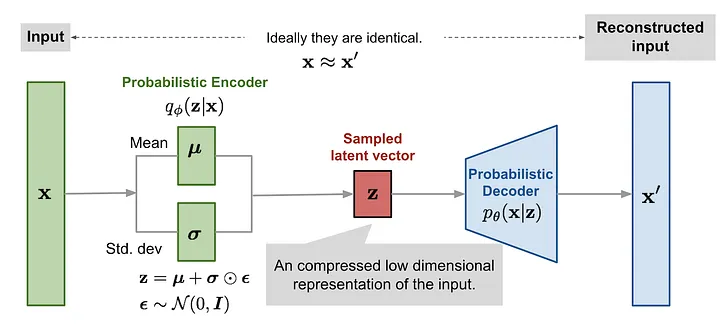
\includegraphics[width=\linewidth]{./imgs/encoder.png}
				\caption{autocodificador}
				\label{fig:autocodificador}
			\end{figure}
			
			Figure \ref{fig:autocodificador} autocodificador.
				
\fi

			Pontos fortes do artigo:
			
			\begin{itemize}
				\item Acompanha código o que facilita a replicação.
			\end{itemize}
			Pontos que o artigo poderia melhorar:
			\begin{itemize}
				\item Muitos termos específicos da área, o que faz com que o artigo seja um pouco inacessível para alguém que está começando os estudos.
			\end{itemize}
			
	\section{Metodologia}
		\subsection{Tipo de Pesquisa}
		O tipo de pesquisa adotado que seguiremos é de experimentação e comparação. Em um primeiro momento testaremos múltiplas técnicas de síntese de voz, tentando entender os desafios para aplicá-las no contexto do português brasileiro e realizaremos a comparação dos resultados.
		
		\subsection{Estudos Selecionados}
		Alguns dos estudos selecionados estão contidos na seção de revisão sistemática da literatura. Atualmente o Estado da arte é o NaturalSpeech \cite{tan2022naturalspeech}, realizaremos experimentações com os modelos de deep learning do tacotron \cite{wang2017tacotron} e de outros estudos a serem definidos.
		
		\subsection{Extração dos dados}
		Para popular os nossa base de dados de vozes, utilizaremos o portal Brasil \footnote{https://gitlab.com/fb-audio-corpora}, mas estamos em busca de outros bancos de vozes disponíveis gratuitamente online para este momento preliminar da pesquisa.

		\subsection{Validação}
		Parte dos nossos estudos iniciais vão ser para entender como validar as nossas experimentações. Alguns dos estudos que já mapeamos utilizam \textit{MOS}, que são métricas subjetivos feitos através de pesquisas com falantes nativos da linguagem. Para fazer a experimentação em si, utilizaremos código aberto das técnicas discutidas no artigo e manipularemos parâmetros de entrada para fazer comparações entre as técnicas e seus resultados. Estudaremos também possibilidades de algoritmos de comparação entre a voz sintetizada e um baseline de voz humana gravada.
	
	\bibliographystyle{ACM-Reference-Format}
	\bibliography{ref}

\end{document}